\documentclass[11pt,border=5pt]{standalone}
\usepackage{fontspec}
\setmainfont{cmunrm.otf}[BoldFont=cmunbx.otf,ItalicFont=cmunti.otf,BoldItalicFont=cmunbi.otf]
\usepackage{amsmath}
\usepackage{unicode-math}
\setmathfont{NewCMMath-Regular.otf}
\usepackage{tikz}
\usetikzlibrary{arrows.meta,patterns,angles,quotes}
\begin{document}
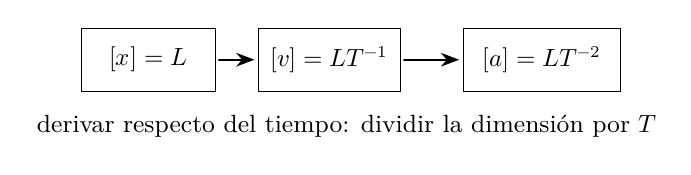
\begin{tikzpicture}[>=Stealth,font=\small,line cap=round,line join=round]
\draw[fill=white] (-2.85,-0.4) rectangle (-1.15,0.4);
\node at (-2,0) {$[x]=L$};
\draw[fill=white] (-0.6000000000000001,-0.4) rectangle (1.2,0.4);
\node at (0.3,0) {$[v]=LT^{-1}$};
\draw[fill=white] (2.0,-0.4) rectangle (4.0,0.4);
\node at (3,0) {$[a]=LT^{-2}$};
\draw[->,thick] (-1.1,0) -- (-0.65,0);
\draw[->,thick] (1.25,0) -- (1.95,0);
\node at (0.5,-0.85) {derivar respecto del tiempo: dividir la dimensión por $T$};

\end{tikzpicture}
\end{document}
